\documentclass{beamer}
\usepackage[utf8]{inputenc}
\usepackage[russian]{babel}
\title{Отчет по второму заданию}
\author{Гудков-Жаданов-Шиков}
\date{15 апреля 2017г.}

\usepackage{natbib}
\usepackage{graphicx}

\begin{document}

\maketitle

\begin{frame}{} 
У нас есть данные за 7 месяцев о количестве произведенных и сломавшихся мечей для каждой из компаний Westeros Inc. и Harpy \& Co. Нам нужно выбрать компанию, мечи которой прослужат дольше. Для этого рассмотрим какая часть мечей у каждой из компаний ломается через 1, 2, ... 6 месяцев после производства. Для начала подсчитаем эту долю для каждого из кузнецов, а затем усредним по компаниям. 
Получим следующие графики для двух компаний:
\end{frame}
\begin{figure}[h!]
\centering
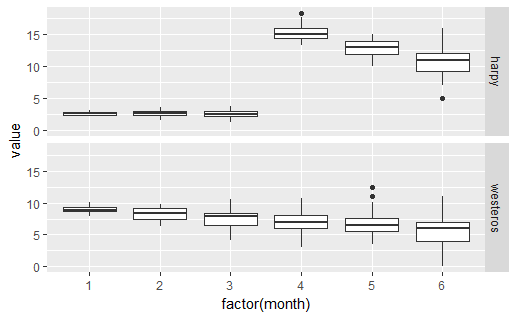
\includegraphics[scale=0.8]{grafik.png}
\caption{Boxplots}
\label{fig:univerise}
\end{figure}
\begin{frame}{} 
Из графика видно, что в первые три месяца мечи Westeros Inc. ломаются чаще мечей Harpy \& Co, но со временем процент ломающихся мечей уменьшается. У компании Harpy \& Co же процент ломающихся мечей резко увеличивается после третьего месяца. И если в отношении Westeros Inc. мы можем предположить что процент мечей ломающихся через n месяцев будет уменьшаться, то для Harpy \& Co мы этого прогнозировать не можем. Так как война будет продолжаться еще целых 11 месяцев, то мы бы рекомендовали контракт заключить с компанией Westeros Inc.
\end{frame}
\begin{frame}
P.S. Если у королевства имеются деньги, и объем производства позволяет менять мечи каждые три месяца, то можно заключить контракт с Harpy \& Co и использовать их мечи по три месяца. Это максимально снизит количество сломаных мечей в бою, что в свою очередь снизит потери воинов в армии.
\end{frame}


\end{document}
